\documentclass[11pt,a4paper]{article}

\usepackage[utf8]{inputenc}
\usepackage[T1]{fontenc}
\usepackage[a4paper,margin=2.5cm]{geometry}
\usepackage[table]{xcolor}
\usepackage{titlesec}
\usepackage{fancyhdr}
\usepackage{enumitem}
\usepackage{tabularx}
\usepackage{longtable}
\usepackage{booktabs}
\usepackage{graphicx}
\usepackage{hyperref}
\usepackage{parskip}
\usepackage{helvet}
\usepackage{amsmath}
\usepackage{amssymb}
\renewcommand{\familydefault}{\sfdefault}

\definecolor{accent}{HTML}{1F4E78}
\definecolor{accentlight}{HTML}{DDEBF7}

\titleformat{\section}{\color{accent}\Large\bfseries}{\thesection.}{0.5em}{}
\titleformat{\subsection}{\color{accent}\large\bfseries}{\thesubsection}{0.5em}{}
\titleformat{\subsubsection}{\color{accent}\normalsize\bfseries}{\thesubsubsection}{0.5em}{}
\titlespacing*{\section}{0pt}{18pt}{8pt}
\titlespacing*{\subsection}{0pt}{14pt}{6pt}

\pagestyle{fancy}
\fancyhf{}
\renewcommand{\headrulewidth}{0.4pt}
\fancyhead[L]{\small Structures polyazot\'ees --- extraction bibliographique}
\fancyhead[R]{\small\thepage}

\hypersetup{colorlinks=true, linkcolor=accent, urlcolor=accent, citecolor=accent}

\title{\color{accent}\textbf{Extraction des structures de compos\'es polyazot\'es\\
\large depuis la bibliographie et g\'en\'eration de fichiers .xyz}}
\author{Pipeline polyN --- biblio\_polyN}
\date{\today}

\begin{document}
\maketitle
\thispagestyle{fancy}

\begin{abstract}
\noindent Ce rapport documente l'extraction syst\'ematique des g\'eom\'etries
mol\'eculaires de compos\'es N$_n$ ($n=2$ \`a $20$, neutres, cations et
anions) rapport\'ees dans deux articles de r\'ef\'erence du dossier
\texttt{biblio\_polyN/}, et leur conversion en fichiers de coordonn\'ees
cart\'esiennes au format \texttt{.xyz}, directement lisibles par le
logiciel de visualisation cristallographique \textbf{VESTA}. Soixante-dix
structures distinctes ont \'et\'e produites. Pour chacune, la m\'ethode de
reconstruction (exacte \`a partir des param\`etres publi\'es, ou topologie
publi\'ee relax\'ee par optimisation GFN2-xTB) est trac\'ee et report\'ee.
\end{abstract}

\section{Sources bibliographiques}

Deux documents du dossier \texttt{biblio\_polyN/} ont \'et\'e d\'epouill\'es
int\'egralement (texte et figures) :

\begin{itemize}
  \item \textbf{[GS]} M.~N.~Glukhovtsev, H.~Jiao, P.~v.~R.~Schleyer,
  \emph{``Besides N$_2$, What Is the Most Stable Molecule Composed Only of
  Nitrogen Atoms?''}, \textit{Inorg. Chem.} \textbf{1996}, \textit{35},
  7124--7133 (fichier \texttt{poly-N.pdf}, 10 pages). Cet article
  (ab initio / DFT, HF, MP2, B3LYP) couvre les isom\`eres de N$_4$, N$_6$,
  N$_8$ (dont l'azidopentazole et l'octaazapentalene, aromatiques), N$_{10}$
  (bispentazole), N$_{12}$ et le dodeca\`edre N$_{20}$.

  \item \textbf{[B]} S.~Fau, M.~Tobita, K.~Wilson, A.~Perera, R.~J.~Bartlett,
  \emph{``Structure and Stability of Polynitrogen Molecules and Their
  Spectroscopic Characteristics''}, Quantum Theory Project, University of
  Florida (fichier \texttt{polynitrogen1.pdf}, 80 pages). Ce rapport
  (B3LYP/aug-cc-pVDZ, avec v\'erifications CCSD(T) pour les esp\`eces les
  plus significatives) recense syst\'ematiquement tous les isom\`eres
  N$_n^{0/\pm}$ trouv\'es li\'es entre $n=2$ et $n=10$, avec structures,
  fr\'equences de vibration, \'energies relatives et enthalpies de
  formation.
\end{itemize}

Pour chaque mol\'ecule, les longueurs de liaison et angles de valence
annot\'es sur les figures de structure ont \'et\'e relev\'es, ainsi que le
groupe ponctuel de sym\'etrie, la multiplicit\'e de spin, la charge et le
niveau de th\'eorie. Lorsque plusieurs niveaux de calcul \'etaient
disponibles pour une m\^eme esp\`ece, la g\'eom\'etrie CCSD(T) (la plus
fiable) a \'et\'e pr\'ef\'er\'ee \`a B3LYP.

\section{M\'ethodologie de reconstruction 3D}

Les figures des deux articles ne donnent, dans l'immense majorit\'e des cas,
que des longueurs de liaison et des angles de valence -- jamais les angles
di\`edres complets (le rapport [B] le pr\'ecise explicitement : \emph{``To
avoid overloading each picture, we have not included the dihedral angles,
which are necessary to completely specify non-planar structures''}). Une
reconstruction rigoureuse des coordonn\'ees cart\'esiennes exige donc une
analyse au cas par cas de la sym\'etrie mol\'eculaire pour d\'eterminer si
ces param\`etres suffisent \`a fixer enti\`erement la g\'eom\'etrie.

\subsection{Niveau 1 --- reconstruction g\'eom\'etrique exacte}

Pour une majorit\'e de structures, le groupe ponctuel annonc\'e implique que
la mol\'ecule est \textbf{plane} (chaines en zigzag C$_s$/C$_2$/C$_{2v}$/C$_{2h}$
dont le mode de vibration ``out-of-plane bend'' confirme la plan\'eit\'e \`a
l'\'equilibre, cycles D$_{nh}$ r\'eguliers ou irr\'eguliers) ou bien
poss\`ede une sym\'etrie assez \'elev\'ee (T$_d$, O$_h$, D$_{3h}$, D$_{2d}$,
I$_h$, D$_{nh}$ pour les prismes) pour que les longueurs de liaison et
angles publi\'es d\'eterminent enti\`erement la structure 3D, sans ambigu\"it\'e
di\`edrale. Dans ces cas (45 structures sur 70), les coordonn\'ees ont
\'et\'e calcul\'ees \textbf{analytiquement} : propagation d'une châine plane
(zigzag), fermeture de cycle, ou constructions de sym\'etrie ferm\'ees
(t\'etra\`edre, cube, prisme droit \'eclips\'e, bipyramide trigonale sans
atome central, cycle \`a 4 plisse D$_{2d}$, paire de cycles reli\'es
perpendiculairement). Un script Python (\texttt{build/geom.py},
\texttt{build/molecules.py}) impl\'emente ces constructions et v\'erifie,
pour chaque liaison publi\'ee, que la distance interatomique reconstruite
correspond \`a la valeur annonc\'ee (\'ecart maximal report\'e dans
\texttt{build/manifest.json}; \'ecarts observ\'es $\le 0{,}15$~\AA,
attribuables aux arrondis des valeurs publi\'ees).

\subsection{Niveau 2 --- topologie publi\'ee, g\'eom\'etrie relax\'ee par GFN2-xTB}

Pour les 25 structures restantes -- cages non planes (``log carrier'',
``book'', ``cap'', ``ladder'', papillon N$_4$, cycles fusionn\'es de type
pentalene ou azulene, cycles \`a 8 non plans de type
cyclooctat\'etra\`ene...) -- les angles di\`edres n\'ecessaires ne sont pas
publi\'es et ne peuvent \^etre d\'eduits de la seule sym\'etrie. La
\textbf{connectivit\'e} (topologie) d\'ecrite dans la r\'ef\'erence a
n\'eanmoins \'et\'e conserv\'ee : une g\'eom\'etrie 3D de d\'epart
raisonnable (cycle(s), chaine ou agr\'egat compact, selon la description
textuelle de la r\'ef\'erence -- voir la colonne ``description'' du tableau
des enthalpies de formation de [B]) est construite, puis relax\'ee par
\textbf{optimisation de g\'eom\'etrie GFN2-xTB} (\texttt{xtb} 6.6.1,
m\'ethode tight-binding semi-empirique d\'ej\`a utilis\'ee par le pipeline
principal de ce d\'ep\^ot, \texttt{polyN\_pipeline.py}), \`a charge et
multiplicit\'e de spin fix\'ees d'apr\`es la r\'ef\'erence. Un pr\'e-passage
GFN-FF (champ de force) est utilis\'e en secours lorsque l'auto-coh\'erence
GFN2 ne converge pas directement depuis le d\'epart g\'en\'erique.

\textbf{Ces 25 structures sont donc illustratives et topologiquement
fid\`eles, mais leurs longueurs de liaison exactes peuvent diff\'erer
l\'eg\`erement des valeurs DFT/CCSD(T) publi\'ees.} Elles sont clairement
identifi\'ees dans le tableau \ref{tab:structures} (colonne ``Statut'') et
dans le commentaire (2\up{e} ligne) de chaque fichier \texttt{.xyz}.

\subsection{Validation}

Chaque structure produite a \'et\'e contr\^ol\'ee automatiquement :
\begin{itemize}
  \item absence de valeurs non-num\'eriques (NaN) ;
  \item distance interatomique minimale $> 0{,}6$~\AA\ (pas de recouvrement
  d'atomes) ;
  \item distance au plus proche voisin $< 2{,}2$~\AA\ pour chaque atome
  (pas de fragment dissoci\'e / atome isol\'e).
\end{itemize}
Les 70 fichiers produits passent ces trois contr\^oles.

\section{Format des fichiers produits}

Chaque fichier \texttt{xyz/<id>.xyz} suit le format standard :
\begin{verbatim}
<nombre d'atomes>
<formule> charge=<q> mult=<2S+1> PG=<groupe ponctuel> | <methode> | src: <reference>
N   x1  y1  z1
N   x2  y2  z2
...
\end{verbatim}
Ce format est import\'e directement par VESTA (\emph{File > Open}, puis
choisir ``.xyz'' comme type de fichier), qui reconna\^it automatiquement
l'esp\`ece atomique (N, et H pour le pentazole neutre) et propose la
repr\'esentation en boules-b\^atons.

\section{R\'esultats}

\subsection{Aper\c{c}u visuel}

La figure~\ref{fig:gallery} montre dix structures repr\'esentatives, de
l'azote mol\'eculaire aux cages les plus complexes.

\begin{figure}[h]
\centering
\begin{tabular}{ccccc}
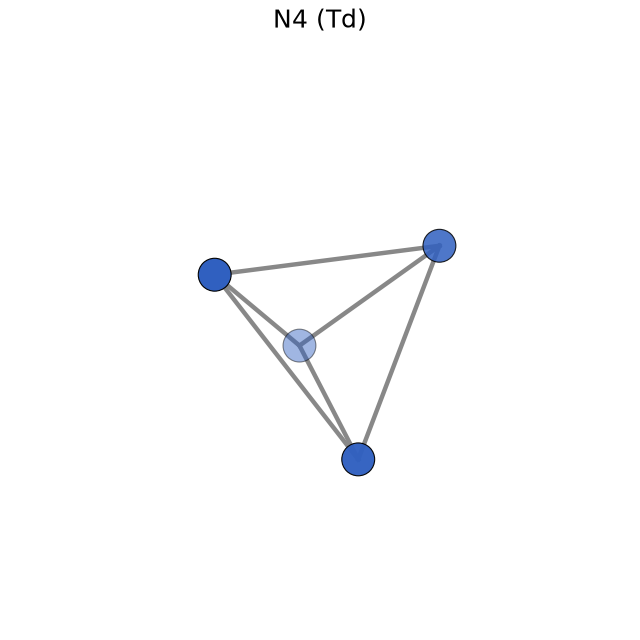
\includegraphics[width=2.6cm]{figures/N4_Td.png} &
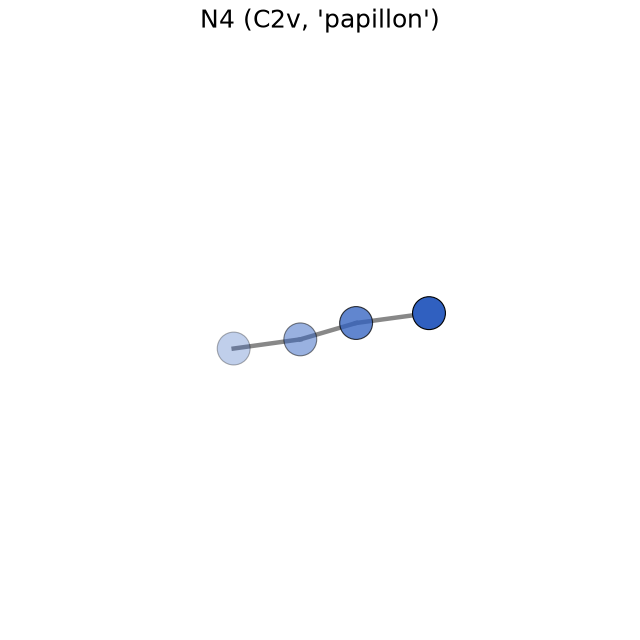
\includegraphics[width=2.6cm]{figures/N4_C2v_butterfly.png} &
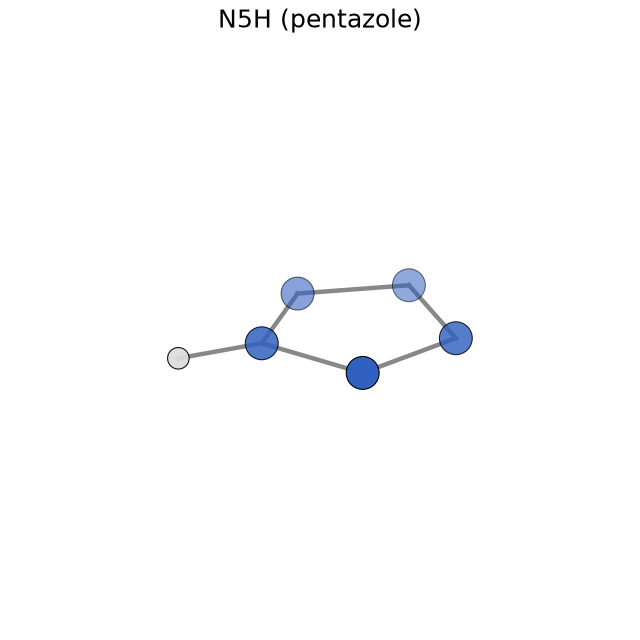
\includegraphics[width=2.6cm]{figures/N5H_pentazole.png} &
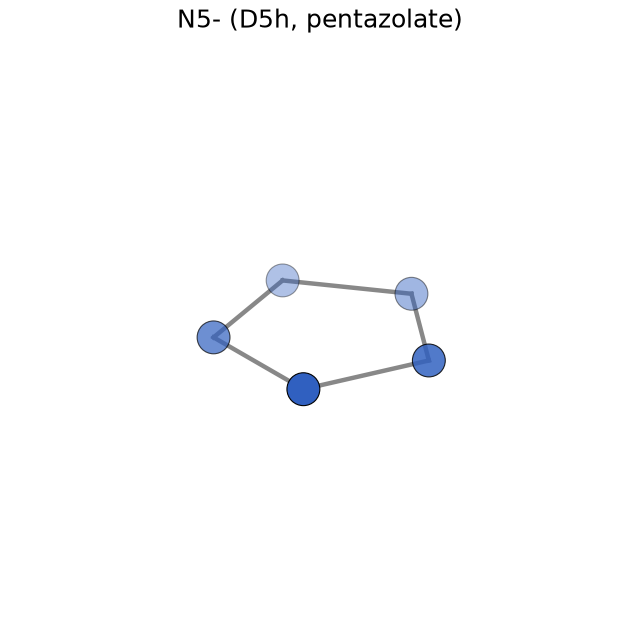
\includegraphics[width=2.6cm]{figures/N5-_pentagon.png} &
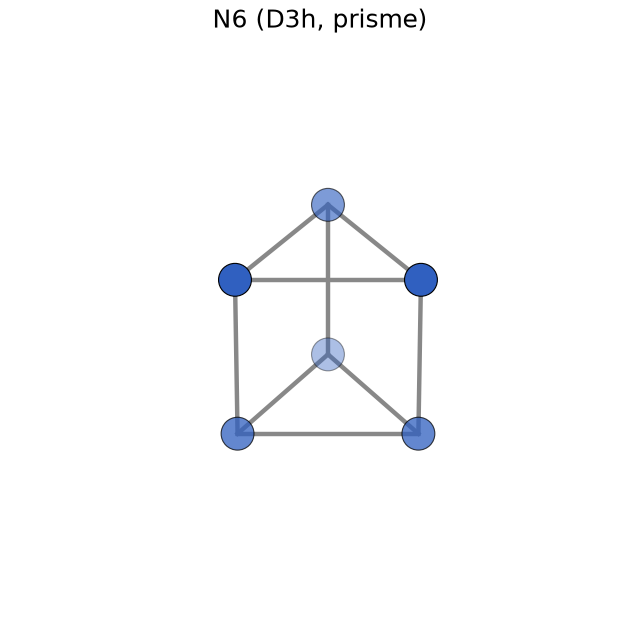
\includegraphics[width=2.6cm]{figures/N6_D3h_prism.png} \\
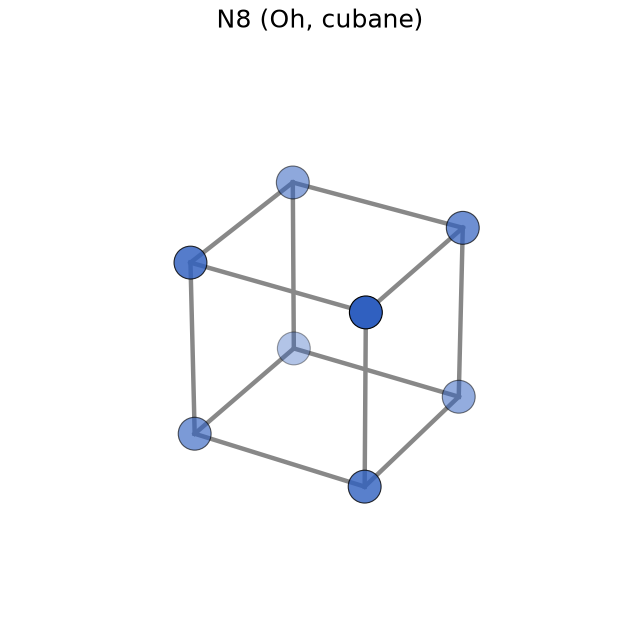
\includegraphics[width=2.6cm]{figures/N8_Oh_cube.png} &
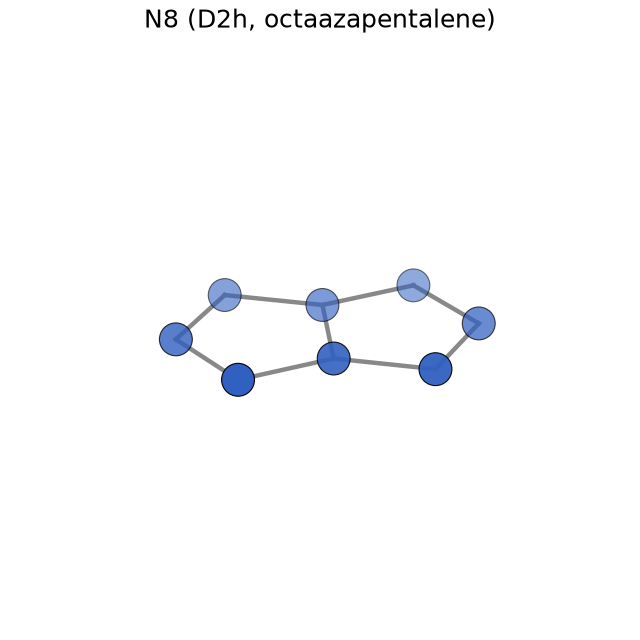
\includegraphics[width=2.6cm]{figures/N8_D2h_pentalene.png} &
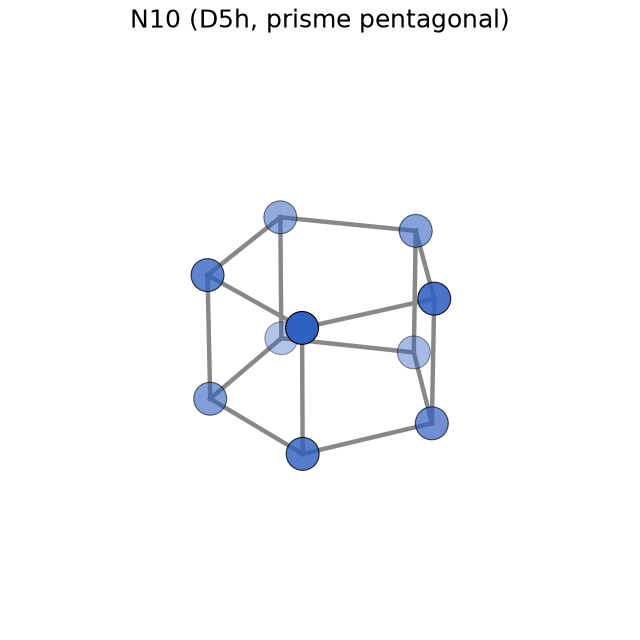
\includegraphics[width=2.6cm]{figures/N10_D5h_prism.png} &
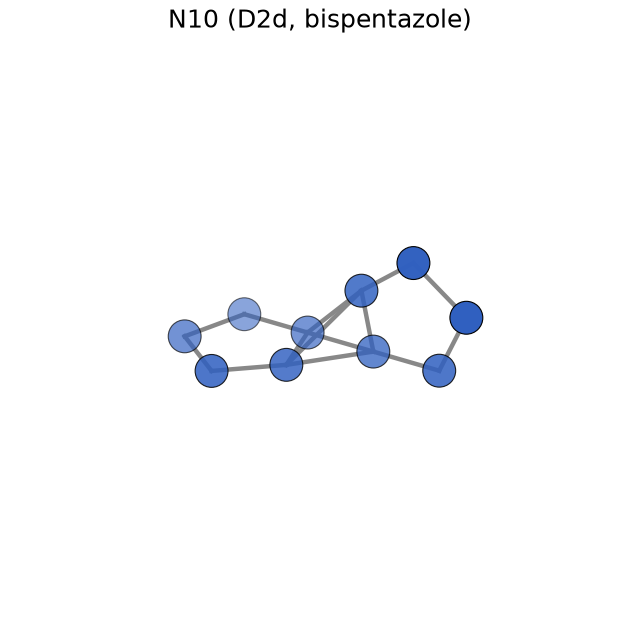
\includegraphics[width=2.6cm]{figures/N10_D2d_linked5rings.png} &
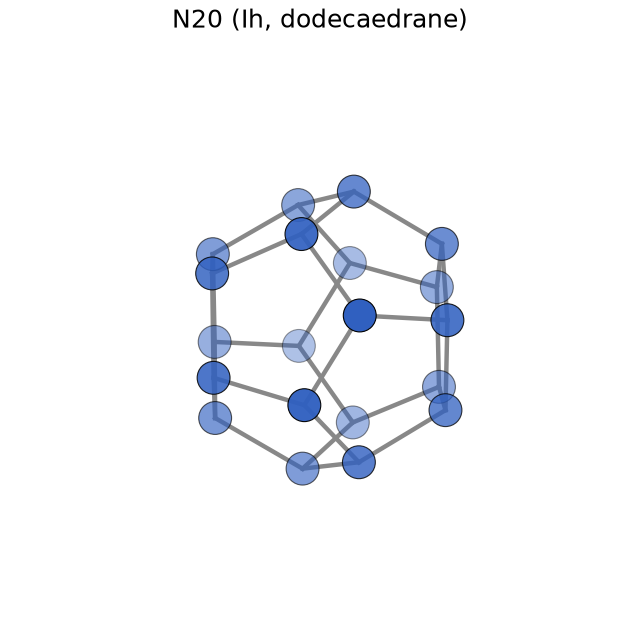
\includegraphics[width=2.6cm]{figures/N20_Ih_dodecahedrane.png} \\
\end{tabular}
\caption{S\'election de dix structures polyazot\'ees reconstruites (rendu
boules-b\^atons simplifi\'e). De gauche \`a droite, de haut en bas :
t\'etraazat\'etra\`edrane N$_4$ (T$_d$), isom\`ere N$_4$ ``papillon''
(C$_{2v}$, relax\'e GFN2-xTB), pentazole N$_5$H, anion pentazolate N$_5^-$
(D$_{5h}$), prisme trigonal N$_6$ (D$_{3h}$), octaazacubane N$_8$
(O$_h$), octaazapentalene N$_8$ (D$_{2h}$, relax\'e GFN2-xTB), prisme
pentagonal N$_{10}$ (D$_{5h}$), bispentazole N$_{10}$ (D$_{2d}$),
dodeca\`edre N$_{20}$ (I$_h$).}
\label{fig:gallery}
\end{figure}

\subsection{Bilan quantitatif}

\begin{center}
\begin{tabular}{lr}
\toprule
Structures reconstruites (total) & 70 \\
\quad dont g\'eom\'etrie exacte (Niveau 1) & 45 \\
\quad dont topologie + relaxation GFN2-xTB (Niveau 2) & 25 \\
Esp\`eces couvertes & N$_2$ \`a N$_{20}$ \\
\'Etats de charge & neutre, cation (+1), anion ($-$1) \\
\bottomrule
\end{tabular}
\end{center}

\subsection{Table compl\`ete des structures}

Le tableau~\ref{tab:structures} liste l'ensemble des 70 fichiers
\texttt{.xyz} produits dans \texttt{biblio\_polyN/xyz/}, avec la formule,
le groupe ponctuel, le niveau de th\'eorie de la g\'eom\'etrie de
r\'ef\'erence et le statut de reconstruction.

\begingroup
\small
\begin{longtable}{@{}p{4.4cm}p{1.3cm}p{1.2cm}p{4.1cm}p{1.9cm}@{}}
\toprule
\textbf{Fichier (id)} & \textbf{Formule} & \textbf{G. ponctuel} & \textbf{Methode} & \textbf{Statut} \\
\midrule
\endhead
\texttt{N2} & N2 & Dinfh & CCSD(T)/aug-cc-pVTZ & exacte \\
\texttt{N2+} & N2$^{+}$ & Dinfh & B3LYP/aug-cc-pVDZ & exacte \\
\texttt{N3+\_linear} & N3$^{+}$ & Dinfh & CCSD(T)/cc-pVTZ & exacte \\
\texttt{N3+\_triangle} & N3$^{+}$ & D3h & CCSD(T)/cc-pVTZ & exacte \\
\texttt{N3-\_bent} & N3$^{-}$ & C2v & B3LYP/aug-cc-pVDZ & exacte \\
\texttt{N3-\_linear} & N3$^{-}$ & Dinfh & CCSD(T)/aug-cc-pVTZ & exacte \\
\texttt{N3-\_triangle} & N3$^{-}$ & D3h & B3LYP/aug-cc-pVDZ & exacte \\
\texttt{N3\_radical} & N3 & Dinfh & B3LYP/aug-cc-pVDZ & exacte \\
\texttt{N4+\_rectangle} & N4$^{+}$ & D2h & B3LYP/aug-cc-pVDZ & exacte \\
\texttt{N4-\_chain\_planar} & N4$^{-}$ & C2h & B3LYP/aug-cc-pVDZ & exacte \\
\texttt{N4-\_rectangle} & N4$^{-}$ & D2h & B3LYP/aug-cc-pVDZ & exacte \\
\texttt{N4\_C2h\_chain} & N4 & C2h & CCSD(T)/aug-cc-pVDZ & exacte \\
\texttt{N4\_D2d\_puckered} & N4 & D2d & CCSD(T)/aug-cc-pVDZ & exacte \\
\texttt{N4\_D2h\_rectangle\_planar} & N4 & D2h & B3LYP/aug-cc-pVDZ & exacte \\
\texttt{N4\_Td} & N4 & Td & CCSD(T)/aug-cc-pVTZ & exacte \\
\texttt{N4\_C2v\_butterfly} & N4 & C2v & CCSD(T)/aug-cc-pVDZ (topologie) & GFN2-xTB \\
\texttt{N5+\_Vchain} & N5$^{+}$ & C2v & CCSD(T)/6-311+G(2d) & exacte \\
\texttt{N5-\_bipyramid} & N5$^{-}$ & D3h & B3LYP/aug-cc-pVDZ & exacte \\
\texttt{N5-\_pentagon} & N5$^{-}$ & D5h & CCSD(T)/aug-cc-pVTZ & exacte \\
\texttt{N6+\_C2h\_planar} & N6$^{+}$ & C2h & B3LYP/aug-cc-pVDZ & exacte \\
\texttt{N6+\_C2v} & N6$^{+}$ & C2v & B3LYP/aug-cc-pVDZ & exacte \\
\texttt{N6-\_Cs\_chain} & N6$^{-}$ & Cs & B3LYP/aug-cc-pVDZ & exacte \\
\texttt{N6\_C2h\_chain} & N6 & C2h & CCSD(T)/cc-pVDZ & exacte \\
\texttt{N6\_D3h\_prism} & N6 & D3h & B3LYP/aug-cc-pVDZ & exacte \\
\texttt{N6+\_C2h\_nonplanar} & N6$^{+}$ & C2h & B3LYP/aug-cc-pVDZ (topologie) & GFN2-xTB \\
\texttt{N6-\_C2\_linked\_triangles} & N6$^{-}$ & C2 & B3LYP/aug-cc-pVDZ (topologie) & GFN2-xTB \\
\texttt{N6\_C2\_book} & N6 & C2 & B3LYP/aug-cc-pVDZ (topologie) & GFN2-xTB \\
\texttt{N6\_D2\_twisted} & N6 & D2 & B3LYP/aug-cc-pVDZ (topologie) & GFN2-xTB \\
\texttt{N7+\_chain} & N7$^{+}$ & C2v & B3LYP/aug-cc-pVDZ & exacte \\
\texttt{N7-\_chain} & N7$^{-}$ & C2v & B3LYP/aug-cc-pVDZ & exacte \\
\texttt{N7\_C2\_linearZZ} & N7 & C2 & B3LYP/aug-cc-pVDZ & exacte \\
\texttt{N7\_C2v\_logcarrier} & N7 & C2v & B3LYP/aug-cc-pVDZ (topologie) & GFN2-xTB \\
\texttt{N7\_Cs\_ring\_chain} & N7 & Cs & B3LYP/aug-cc-pVDZ (topologie) & GFN2-xTB \\
\texttt{N8-\_C2h\_ZEZ} & N8$^{-}$ & C2h & B3LYP/aug-cc-pVDZ & exacte \\
\texttt{N8-\_C2h\_chain} & N8$^{-}$ & C2h & B3LYP/aug-cc-pVDZ & exacte \\
\texttt{N8\_C1\_ZZE} & N8 & C1 & B3LYP/aug-cc-pVDZ & exacte \\
\texttt{N8\_C2h\_EEE} & N8 & C2h & B3LYP/aug-cc-pVDZ & exacte \\
\texttt{N8\_C2h\_ZEZ} & N8 & C2h & B3LYP/aug-cc-pVDZ & exacte \\
\texttt{N8\_C2v\_EZE} & N8 & C2v & B3LYP/aug-cc-pVDZ & exacte \\
\texttt{N8\_Oh\_cubane\_GS} & N8 & Oh & Becke3LYP/6-31G* & exacte \\
\texttt{N8\_Oh\_cube} & N8 & Oh & B3LYP/aug-cc-pVDZ & exacte \\
\texttt{N8\_C2h\_ladder} & N8 & C2h & B3LYP/aug-cc-pVDZ (topologie) & GFN2-xTB \\
\texttt{N8\_C2v\_branched} & N8 & C2v & B3LYP/aug-cc-pVDZ (topologie) & GFN2-xTB \\
\texttt{N8\_C2v\_ring} & N8 & C2v & B3LYP/aug-cc-pVDZ (topologie) & GFN2-xTB \\
\texttt{N8\_Cs\_ZEE} & N8 & Cs & B3LYP/aug-cc-pVDZ (topologie) & GFN2-xTB \\
\texttt{N8\_Cs\_azidopentazole} & N8 & Cs & Becke3LYP/6-31G* (topologie) & GFN2-xTB \\
\texttt{N8\_Cs\_pentagonal} & N8 & Cs & B3LYP/aug-cc-pVDZ (topologie) & GFN2-xTB \\
\texttt{N8\_D2d\_octaazacyclooctatetraene} & N8 & D2d & Becke3LYP/6-31G* (topologie) & GFN2-xTB \\
\texttt{N8\_D2h\_pentalene} & N8 & D2h & B3LYP/6-31G* (topologie exacte, geometrie relaxee GFN2-xTB) & GFN2-xTB \\
\texttt{N8\_D2h\_ring\_pendant} & N8 & D2h & B3LYP/aug-cc-pVDZ (topologie) & GFN2-xTB \\
\texttt{N9+\_chain} & N9$^{+}$ & C2v & B3LYP/aug-cc-pVDZ & exacte \\
\texttt{N9-\_chain} & N9$^{-}$ & C2v & B3LYP/aug-cc-pVDZ & exacte \\
\texttt{N9-\_chain\_twistedW} & N9$^{-}$ & C2 & B3LYP/aug-cc-pVDZ & exacte \\
\texttt{N9\_chain} & N9 & C2v & B3LYP/aug-cc-pVDZ & exacte \\
\texttt{N9+\_fused\_rings} & N9$^{+}$ & C2v & B3LYP/aug-cc-pVDZ (topologie) & GFN2-xTB \\
\texttt{N9-\_ring\_chain} & N9$^{-}$ & Cs & B3LYP/aug-cc-pVDZ (topologie) & GFN2-xTB \\
\texttt{N9\_fused\_rings} & N9 & C2v & B3LYP/aug-cc-pVDZ (topologie) & GFN2-xTB \\
\texttt{N10+\_chain} & N10$^{+}$ & C1 & B3LYP/aug-cc-pVDZ & exacte \\
\texttt{N10\_D10h\_ring} & N10 & D10h & Becke3LYP/6-31G* & exacte \\
\texttt{N10\_D2d\_bispentazole\_GS} & N10 & D2d & Becke3LYP/6-31G* & exacte \\
\texttt{N10\_D2d\_linked5rings} & N10 & D2d & B3LYP/6-31G* & exacte \\
\texttt{N10\_D5h\_prism} & N10 & D5h & B3LYP/aug-cc-pVDZ & exacte \\
\texttt{N10+\_rings} & N10$^{+}$ & C1 & B3LYP/aug-cc-pVDZ (topologie) & GFN2-xTB \\
\texttt{N10-\_D2h\_perp\_rings} & N10$^{-}$ & D2h & B3LYP/aug-cc-pVDZ (topologie) & GFN2-xTB \\
\texttt{N10\_C3\_cap} & N10 & C3 & B3LYP/aug-cc-pVDZ (topologie) & GFN2-xTB \\
\texttt{N10\_Cs\_ring\_chain} & N10 & Cs & B3LYP/aug-cc-pVDZ (topologie) & GFN2-xTB \\
\texttt{N10\_cage\_C2v} & N10 & C2v & B3LYP/aug-cc-pVDZ (topologie) & GFN2-xTB \\
\texttt{N12\_C2h\_dipentazolyldiazene} & N12 & C2h & Becke3LYP/6-31G* (topologie) & GFN2-xTB \\
\texttt{N20\_Ih\_dodecahedrane} & N20 & Ih & Becke3LYP/6-31G* & exacte \\
\texttt{N5H\_pentazole} & N5H & C2v & MP2(fc)/6-31G* & exacte \\
\bottomrule
\end{longtable}

\endgroup
\label{tab:structures}

\section{Limites connues}

\begin{itemize}
  \item Les 25 structures ``GFN2-xTB'' du tableau reproduisent la
  \textbf{connectivit\'e} d\'ecrite dans la r\'ef\'erence mais pas
  n\'ecessairement, au sens strict, la conformation di\`edrale exacte du
  minimum DFT/CCSD(T) publi\'e (non document\'ee dans les figures sources).
  \item Quelques cycles annonc\'es \textit{presque plans} pr\'esentent un
  tr\`es faible r\'esidu de fermeture (jusqu'\`a $\sim0{,}1$~\AA\ pour le
  pentazole N$_5$H) attribuable aux arrondis \`a 1--2 d\'ecimales des
  angles publi\'es dans les figures sources.
  \item La longueur de liaison N--H du pentazole neutre (N$_5$H) n'\'etant
  pas indiqu\'ee dans [GS], une valeur standard de 1{,}00~\AA\ a \'et\'e
  utilis\'ee.
  \item Les structures marqu\'ees GFN-FF (secours) dans
  \texttt{build/manifest.json} n'ont pas converg\'e en GFN2-xTB final ; leur
  g\'eom\'etrie provient du champ de force GFN-FF uniquement, l\'eg\`erement
  moins pr\'ecis que GFN2.
\end{itemize}

\section{Reproductibilit\'e}

L'ensemble de la cha\^ine de production est scriptable et rejouable depuis
\texttt{biblio\_polyN/build/} :
\begin{verbatim}
python3 build/main.py           # regenere tous les .xyz + build/manifest.json
python3 build/render.py         # regenere les figures PNG
python3 build/make_table_tex.py # regenere table_structures.tex
pdflatex rapport_polyN_biblio.tex
\end{verbatim}
La base de donn\'ees des param\`etres g\'eom\'etriques extraits des deux
articles (longueurs de liaison, angles, groupe ponctuel, m\'ethode,
r\'ef\'erence page par page) est enti\`erement lisible dans
\texttt{build/molecules.py}.

\section{Conclusion}

Cette extraction fournit un jeu homog\`ene de 70 structures polyazot\'ees
N$_2$--N$_{20}$ au format \texttt{.xyz}, directement exploitables dans
VESTA pour la visualisation, ou comme g\'eom\'etries de d\'epart pour le
pipeline \texttt{polyN\_pipeline.py} de ce d\'ep\^ot (optimisation
GFN2-xTB, v\'erification de fr\'equences, enveloppes convexes de
stabilit\'e). Les structures marqu\'ees comme reconstruites exactement
peuvent \^etre consid\'er\'ees comme fid\`eles aux g\'eom\'etries publi\'ees
dans [GS] et [B] ; les autres constituent des mod\`eles topologiquement
corrects mais g\'eom\'etriquement approximatifs, faute d'information
di\`edrale disponible dans les sources.

\end{document}
